\section{The A3-E Model}\label{sec:proposal}

\begin{figure}[tbp]
	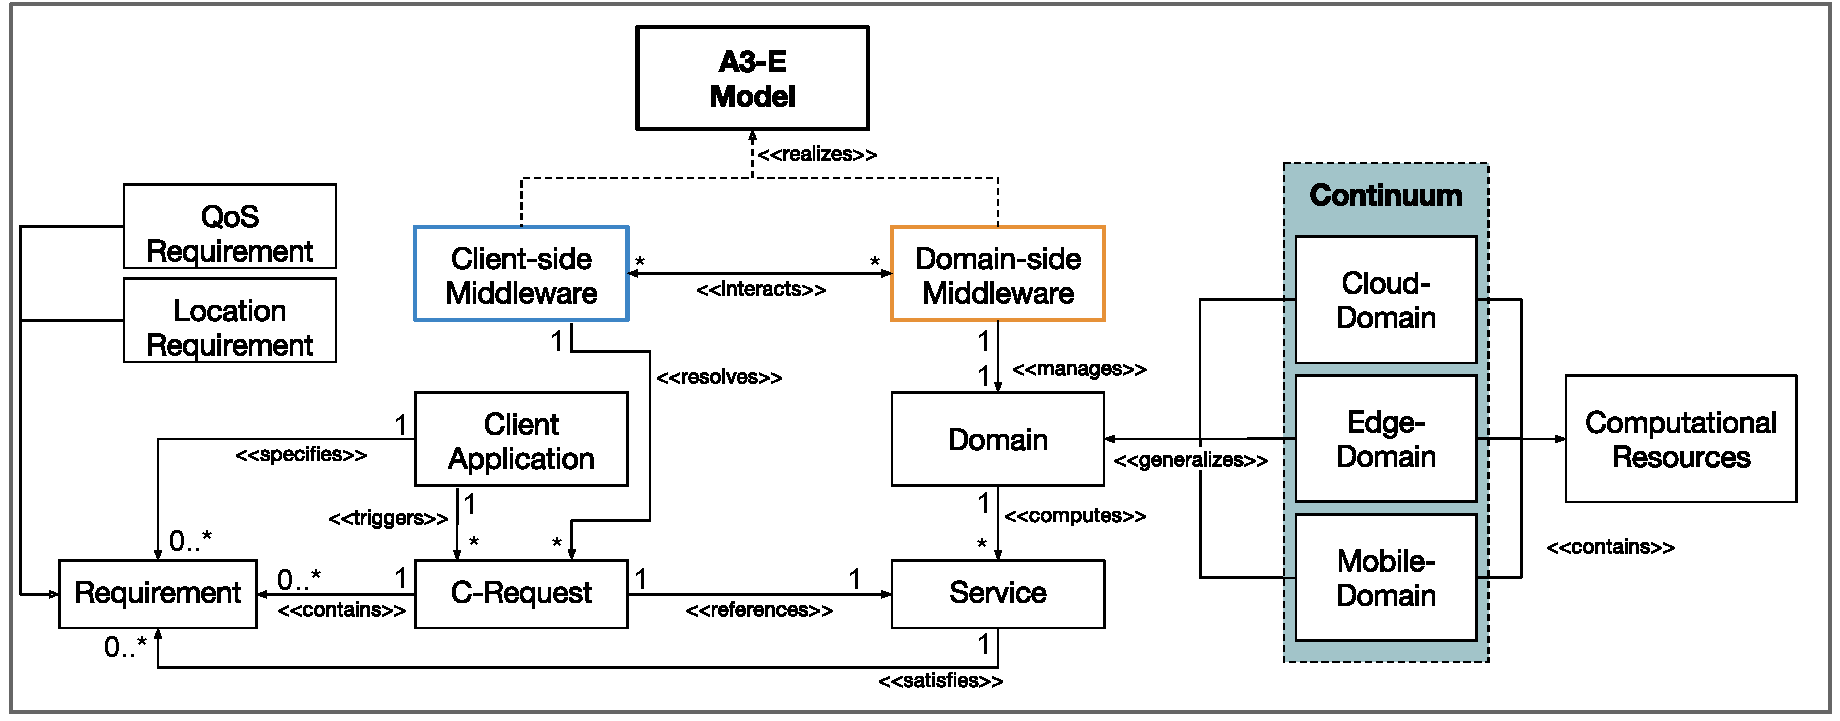
\includegraphics[width=1\textwidth]{figs/A3-E-model.pdf}
	\caption{The A3-E Model.}
	\label{fig:A3-E-model}
\end{figure}

As depicted in Fig.~\ref{fig:A3-E-model}, the A3-E model consists of the different concepts and mechanisms required for the realization of the cloud-edge-mobile continuum. Its name inherits from the four phases process -- namely, \textit{(\textbf{A}wareness), (\textbf{A})cquisition, (\textbf{A})llocation, and (\textbf{E})ngagement} -- employed both by clients and the different types of computational resources composing the continuum. 

The A3-E model also encompasses the concepts of client applications, services, requirements, as well as those of a client-side and a domain-side middleware, both implementing the A3-E process. In specific, the client middleware is responsible for handling client application requests and forwarding them to the domain that best satisfies the client application requirements.  In turn, the domain middleware is responsible for the self-management of services life-cycle in a given domain. Last but not least, the constituents of the continuum (i.e., cloud datacenters, edge servers, and mobile devices) are respectively represented in the model by the cloud-domain, edge-domain, and mobile-domain. Each domain contains its own and potentially heterogeneous pool of computational resources.

\subsection{A3-E Process: Phases}\label{sec:A3-E-process}

%What: the process within A3-E
The A3-E process is composed of four phases. Each phase encompasses activities -- performed by the client-side and domain-side middlewaress -- that take care of specific concerns in the interaction among client applications and the compute continuum. The process provides flexibility with respect to its phases in order to addresses the particularities of the continuum constituents. Next, we describe the four phases depicted in Fig.~\ref{fig:A3-E-process}, which represents an instance with the complete process. Later on, other possible instances of the A3-E model are mapped to distinct scenarios of the compute continuum.

%Next, the four A3-E phases are further described and mapped to the requirements elicited in  Section~\ref{sec:requirements}. Later on, other possible instances of the A3-E model are correlated with scenarios of the compute continuum.

\subsubsection*{Engagement Phase}\label{sec:A3-E-engagement}

The \textit{engagement} phase models the actual interaction between a client and a service in the continuum. At this stage of the client-domain interaction, the requested service must be already deployed by the domain hosting the service(s).  Moreover, the client must have selected this domain for consuming its service(s). In order to overcome the heterogeneity of the continuum and enable inter-operation, A3-E adheres to the use of service-orientation in which clients engage with remove services by means of a request/response protocol (e.g., RESTful services over HTTP).

%For instance, traditional cloud-based services are pre-allocated. In the later case, the remaining A3-3 phases are not employed. Nonetheless, in other scenarios of the continuum --- specially those with resource limitations --- a dynamic and opportunistic allocation shall improve the efficiency in which domain resources are consumed.

\begin{figure}[tbp]
	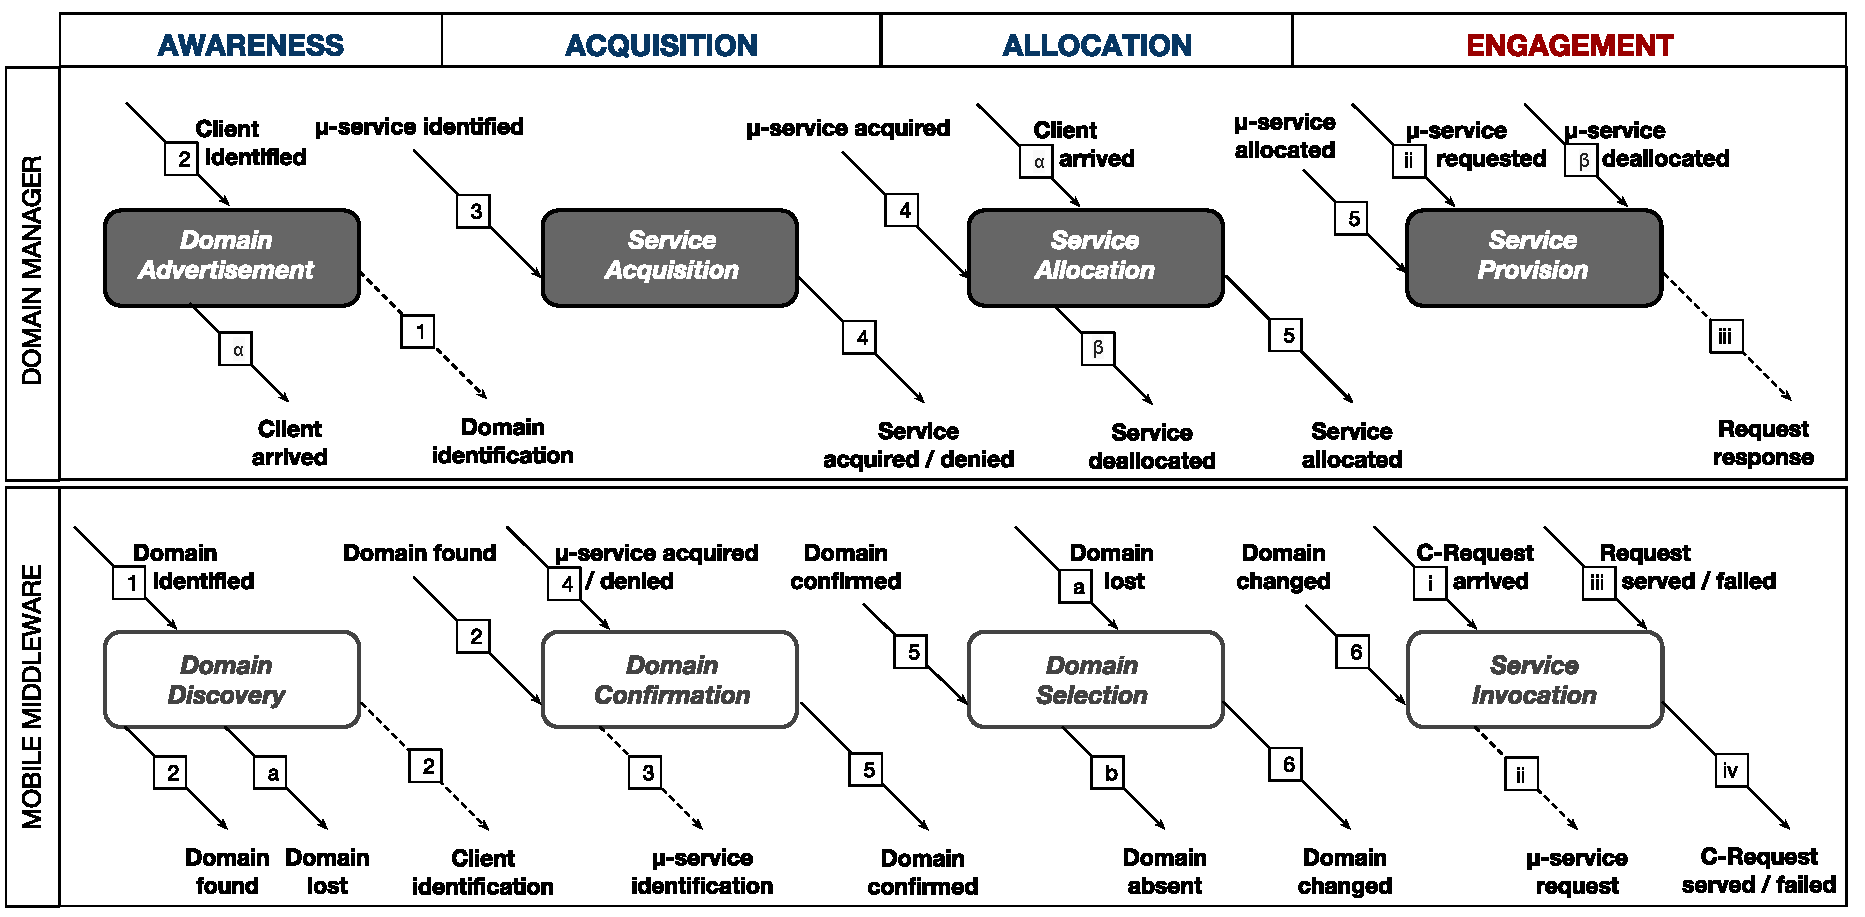
\includegraphics[width=0.95\textwidth]{figs/A3-E-process}
	\caption{The A3-E Process. Phases are delimited by vertical lines and the main activity of each phase by the label within each phase; labels within parenthesis represent the states of a domain to a client (and vice-versa)}
	\label{fig:A3-E-process}
\end{figure}

\subsubsection*{Allocation Phase}\label{sec:A3-E-allocation}

The allocation phase has the following purposes: 1) to enable the efficient (Req. \textbf{R1.1}) and automated (Req. \textbf{R3.1}) allocation of domains' computational resources; and to enable clients to choose the best candidate among different available domains (Req. \textbf{R2.1}).

%cloud providers already implement automated scaling mechanisms, e.g, with the allocation of virtual machines and container instances on demand. 

From the domains perspective, A3-E addresses efficiency by adhering to the FaaS execution model in which stateless functions can be deployed and scaled on demand without minimum pre-allocation of resources. In particular, the allocation phase is modeled by a self-management loop~\cite{kephart2003vision} (Fig.~\ref{fig:service-allocation-loop}) in which computational resources are allocated and deallocated according to: a) the monitored QoS os services provided by the domain; and b) the SLA between the domain provider and client applications. 

%2) the allocation policy employed by the domain; and 3) the availability of resources. 

%For instance, an edge-domain could feature two main SLA categories: one for critical applications (e.g., connected vehicles) providing higher priority and availability of services; and another for non-critical applications (e.g., augmented reality) providing opportunistic services based on the availability of resources in the domain. Depending on the policy (Section~\ref{sec:A3-E-policies}), 

From the clients perspective, the allocation phase refers to the selection, at a specific context, of the domain that best suits its requirements from a list of available domains and respective QoS attributes. The later must be updated as part of a self-management control loop (Fig.~\ref{fig:domain-selection-loop}) in which the client checks for the QoS levels of each available domain and decides for the alternative that best satisfies its requirements. 

%For instance....

%From the client-side, once the awareness phase has been active and identified the current alternative domains, the client may consider QoS values from each domain to make the decision of which one to engage. Conversely, the lack of awareness implies that client engagement with a specific domain must be solved by means of a well-known name. In the later case, the network backbone is responsible for routing client requests to specific domains.


\begin{figure}[tbp]
	\centering
	\captionsetup[subfigure]{width=0.4\textwidth}	
	\null\hfill
	\subfloat[Services allocation control loop; domains must monitor the QoS of deployed services and adapt its allocation scheme to prevent SLA violation.\label{fig:service-allocation-loop}]{ 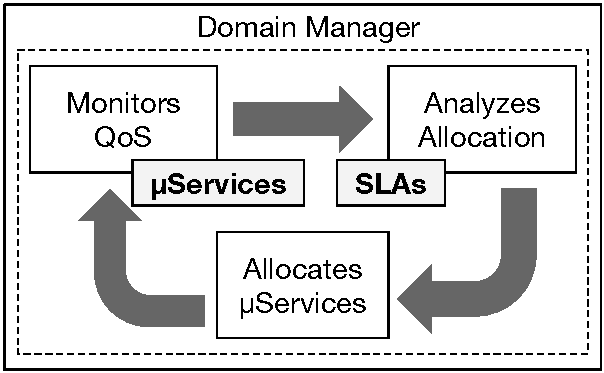
\includegraphics[width=0.4\textwidth]{figs/service-allocation-loop}}
	\captionsetup[subfigure]{width=0.4\textwidth}	
	\hfill
	\subfloat[Domain selection control loop; clients must monitor available domains and select the one that best satisfies its requirements.\label{fig:domain-selection-loop}] {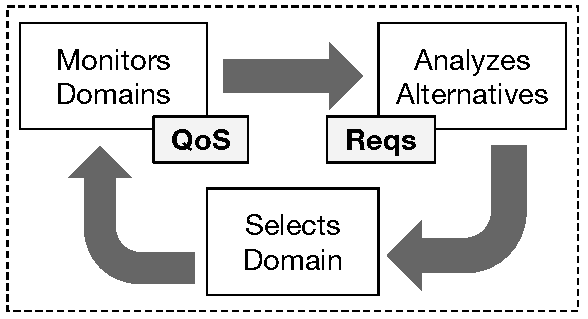
\includegraphics[width=0.4\textwidth]{figs/domain-selection-loop}}
	\hfill\null
	\caption{Self-management control loops for service allocation and domain selection}\label{fig:allocation-loops}
\end{figure}

\subsubsection*{Acquisition Phase}\label{sec:A3-E-acquisition}

The Acquisition phase has the following purposes: 1) to enable the efficient (Req. \textbf{R1.2}) and automated (Req. \textbf{R3.2}) download and installation of service artifacts; and 2) to enable clients to identify, among the known domains, those compatible with their requirements (Req. \textbf{R2.1}).

From the domains perspective, A3-E furthers improve the efficiency of resource usage with the dynamic acquisition of service artifacts. In specific, this phase is modeled by the download and installation of artifacts upon identification of requirements from a given application. 
%In case the service has already been acquired or as the acquisition finishes, clients should add that domain to their list of available domains. 
From the clients perspective, acquisition is modeled by the simple addition of a domain to a list of available domains.

%From the domain side, the lack of acquisition implies that service assets must be previously made available. Nonetheless, the preliminary acquisition of a large number of assets is limited by the domain storage capability. 

%Conversely, the automated and opportunistic acquisition of service assets improves storage efficiency with the cost of a setup time $\Delta_{AQ}$. For instance, domains that become aware of clients' requirements may pro-actively start the acquisition phase and become ready for allocation before the first service request arrives.

%otherwise, domains must rely on the detection of a first service request or some other triggering condition to start the acquisition phase and, after setup time $\Delta_A$, become ready for allocation. 


\subsubsection*{Awareness Phase}\label{sec:A3-E-awareness}


%Why do we need awareness?
%CA: awareness is not needed because the edge domain should always be coupled to the network infrastructure; network components shoudl aways route traffic to existing edge servers; additionally, the edge domain should be able to acquire and allocate services upon detection of the first requests.  
%A: A3-E model is agnostic w.r.t. the use of network technologies to route traffic to the edge servers; a given domain my count on network components to traffic route to its servers instead of negociating directly with clients aware of its existance; nonetheless, the lack of awareness limits the acquisition and deployment of services to reactive, as the domain would only identify a given service upon the first request has been made. Clients, in the other hand, would not be able to choose from alternative domains. 

Finally, the Awareness phase has the following purposes: 1) to enable domains to pro-actively initialize the acquisition and allocation phases based on its 
awareness of applications whose hosting devices happens to be in the domain coverage area (Req.~\textbf{R2.3}); and 2) to enable clients to discover the address of local domains (Req.~\textbf{R2.2}).

From the domains perspective, the awareness of clients presence in their coverage area allows a proactive download and installation of services artifacts (acquisition phase) and/or the allocation of services (allocation phase) potentially before a first request to that service arrives, alleviating the delay introduced by services setup.  From the clients perspective, the awareness phase increases the range of alternatives from the continuum that can be used to satisfy their requirements.

%Such behavior allows that are opportunistically acquired and/or allocated to mitigate their setup delay by triggering these phases upon awareness of client(s) in their coverage area.

%From the domain side, the lack of awareness of clients in the domain coverage area prevents triggering the acquisition and subsequently allocation phases based on this event. From the client side, the lack of awareness from surrounding domains prevents them to make the decision of which domains to use. In the later case, clients must rely on external components to reach servers (e.g., traffic managers and DNS servers).

\subsection{Concrete Scenarios}

\begin{center}
	\begin{table}[htbp]
		\small
		\caption{Domain-side instances of the A3-E model corresponding to parts of the cloud-edge-mobile continuum (CTN) with corresponding execution model (E.M.), awareness mechanisms (\textbf{W}ell-\textbf{K}nown-\textbf{N}ame or \textbf{A}dvertisement\&\textbf{D}iscovery), and policies (\textbf{P}roactive, \textbf{S}equential, \textbf{R}eactive) that may be employed for triggering the acquisition and allocation in each instance. }\label{tab:A3-E-instances}
		\begin{tabular}{ c c c c c c }
			\toprule
			
			CTN & E.M. & \textbf{A}WARENESS & \textbf{A}CQUISITION	& \textbf{A}LLOCATION 	& \textbf{E}NGAGEMENT  	\\
			
			\midrule
			
			\multirow{2}{*}{ Cloud }
			& IaaS	& W.K.N.	& OFFLINE		& HOT-START	& BY REQUEST\\
			& FaaS		& W.K.N.	& OFFLINE		& COLD-START	& BY REQUEST\\\midrule					
			\multirow{2}{*}{ Edge }
			& FaaS		& W.K.N.	& [P, R]		& [P, S, R] 	& BY REQUEST\\
			& FaaS		& A\&D	& [P, S, R]		& [P, S, R]		& BY REQUEST\\\midrule	
			\multirow{1}{*}{ Mobile }
			& FaaS	& LOCAL  & OFFLINE	& HOT-START 	& BY REQUEST\\
			
			\bottomrule
		\end{tabular}
	\end{table}
\end{center}
\normalsize

Table~\ref{tab:A3-E-instances} correlates the possible domain-side instances of the A3-E model with different parts of the cloud-edge-mobile continuum along with the approach used for awareness and the policies~\footnote{The policy adopted by a phase affects which policies may be adopted by its subsequent phase (e.g., a reactive acquisition implies a reactive allocation, as service assets must first be acquired before been deployed, whilst a proactive acquisition may be combined with a reactive allocation).} depicted in Fig.~\ref{fig:A3-E-domain} that may be adopted in each case. 

By taking into account the conflicting properties of \textit{efficiency} and \textit{delay}, we envision the following mapping between A3-E instances and concrete scenarios composing the cloud-edge-mobile continuum:

--- \textbf{Cloud-IaaS}. Services hosted in the cloud are, in most of the cases, reachable by means of a well-known Internet name (therefore, no dynamic awareness is employed). Assets used by these services are preliminarily deployed to cloud servers (thus, no dynamic acquisition is employed). Virtual machines and containers are pre-allocated (hot start), and cloud's elasticity mechanisms take care of the (de)allocation of resources according to a service level agreement (SLA). Finally, cloud services are invoked by clients (engagement phase). Target services: delay-tolerant and stateful computation; persistence.

--- \textbf{Cloud-FaaS}. The FaaS model distinguishes from the cloud instance described above by enforcing the use of stateless functions that can be quickly allocated for execution without minimum pre-allocation (cold start). Targeted services: delay-tolerant and stateless computation.

--- \textbf{Edge-Opportunistic}. Services hosted in the edge, in contrast, may need to opportunistically advertise their existence (awareness phase), acquire application assets (acquisition phase), make them ready for invocation (allocation phase), before finally been able to expose the required computation as services to be consumed. In this case, the policies employed for acquisition and allocation may vary between proactive, sequential, or reactive. Targeted services: non-critical applications with desirable requirements for low-latency.

--- \textbf{Edge-Critical}. The later modality of edge computing may co-exist with others in which: 1) services are transparently accessed through well-known Internet names; 2) service assets are pre-acquired (offline acquisition); and 3) services are pre-allocated in order to increase the readiness required by certain types of applications (hot start). Targeted services: critical applications with strict requirements for low-latency.

--- \textbf{Mobile}. This last instance represents the local computation performed by mobile devices. It provides a zero network latency with high availability; in contrast, the resource constraints of mobile devices may result in lower processing performance and undesirable battery drain, therefore justifying the use of other instances (mobile computation offloading), unless none is available. Targeted services: latency-sensitive and lightweight computation.

%TBW: Example with one of the applications mentioned in the motivation (AR/CV).

\subsection{Reference Architecture}

\begin{figure}[tbp]
	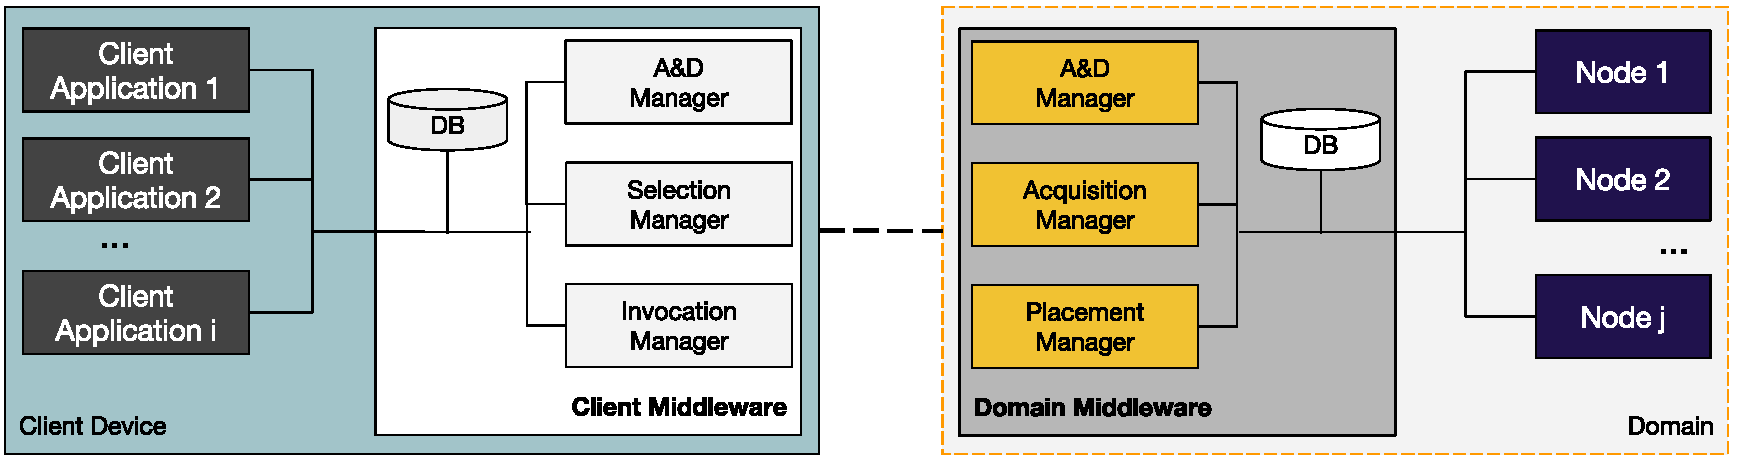
\includegraphics[width=.95\textwidth]{figs/A3-E-reference-architecture}
	\caption{A3-E architecture in Mobile Devices and Edge Domains}
	\label{fig:reference-architecture}
	\end{figure}
	
TOOD: describe